\section{Prototype}
    After one year of research, implementation and trials with error, the game prototype ends up with following functionalities.
    Images below represent how the game scene went through a long process of changes to end up in a functional state.
	\begin{enumerate}
        \item Player First Person (FP) view through SteamVR prefab with the attached camera.
        \item Two HTCVive controllers, capable of providing simple user input.
        \item Tank object provided by PhD candidate, who supported research by providing a prefab of his Bachelor final year work. 
        \item Spherical texture, representing the movie scene, with the reversed shader.
        An object capable of output a proper 360 video stream inside the game.
        \item A canvas video appearing in front of the players view to summarise relevant information.
        \item Few spherical objects acted as markers for target detection.
    \end{enumerate}
	This project is a continuation from the researcher, who established a ground for a continuous video stream.
    Based on the result of his work, a 360degree camera video stream has been integrated before into the Unity game engine.
    His work used a sky-box environment build to create a realistic world. However, the current one relies on video conversion and streaming through \textit{MovieTexture}.
    To resolve the detection problem of the code with finding tanks and colours, it went through several implementations.
    The first implementation consisted of 5 out of 6 plates, surrounded tank from all directions, except the bottom, as shown in subfigure~\ref{fig:oldScene1}.
    Later, the environment got redeveloped into something more functional.
    As a result, a spherical object surrounded a player with only half of the size, creating a hemisphere.
	\begin{figure}[H]
		\centering
		\begin{subfigure}[b]{0.4\textwidth}
			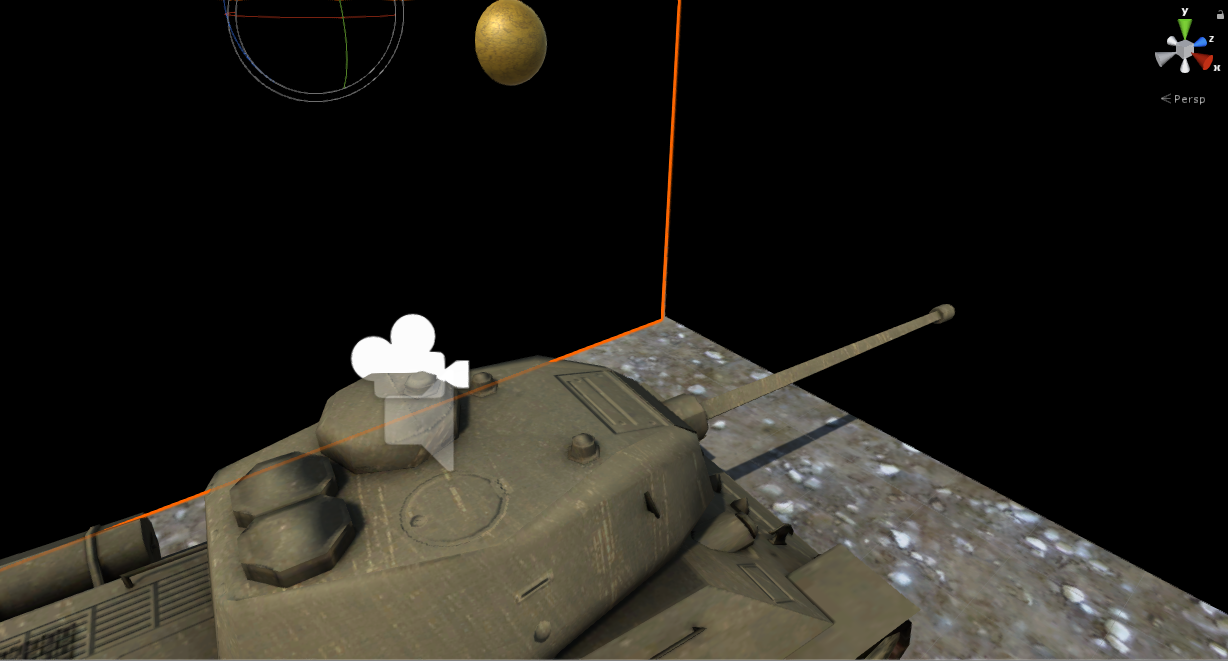
\includegraphics[width=\linewidth]{project/images/scene1.PNG}
			\caption{Changing view between tank and turret}
			\label{fig:oldScene1}
		\end{subfigure}
		\begin{subfigure}[b]{0.4\textwidth}
			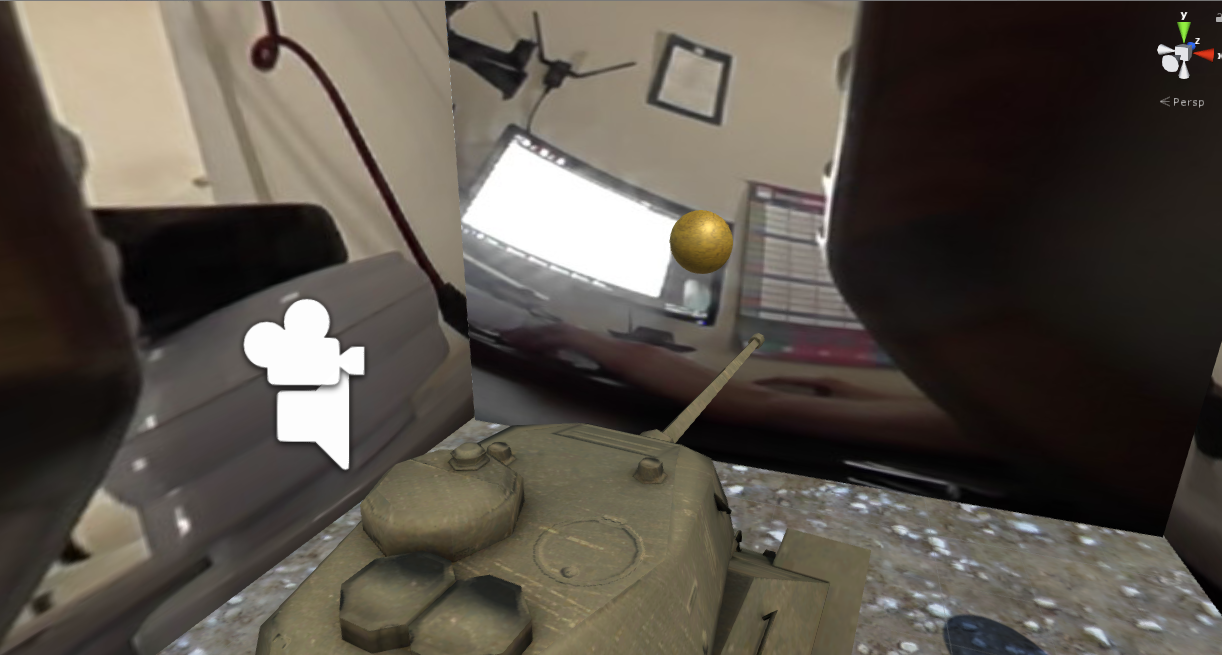
\includegraphics[width=\linewidth]{project/images/scene2.PNG}
			\caption{Entering Tank view screen}
			\label{fig:oldSscene2}
		\end{subfigure}
		\caption{Images from Unity base of development}\label{fig:scene-developemt}
	\end{figure}
	%%%%%%% Figure required reordering
	\begin{figure}[H]
    	\centering
    	\begin{subfigure}[b]{0.4\textwidth}
    		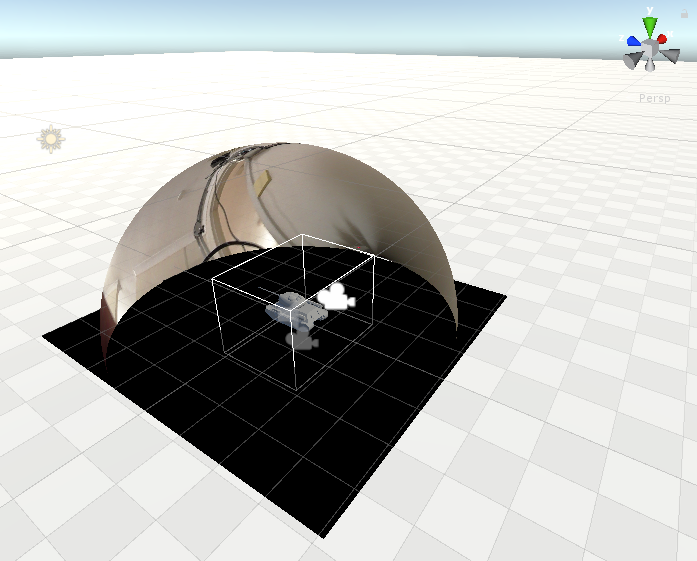
\includegraphics[width=\linewidth]{project/images/newLook2.PNG}
    		\caption{New representation of test area}
    		\label{fig:newScene1}
    	\end{subfigure}
    	\begin{subfigure}[b]{0.4\textwidth}
    		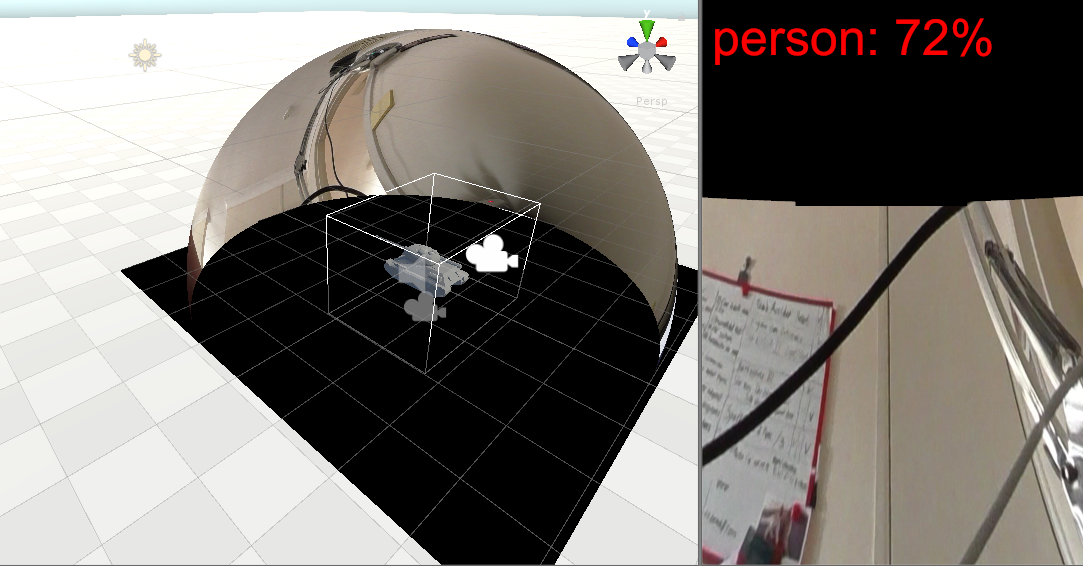
\includegraphics[width=\linewidth]{project/images/recognition.PNG}
    		\caption{Test Human recognition}
    		\label{fig:newScene2}
    	\end{subfigure}			
    	\caption{Images from Unity second base of usage}\label{fig:scene-developemt}
    \end{figure}
	As soon as the game starts, the texture produces the output of camera simulating realistic surrounding area.
    Subfigure~\ref{fig:newScene2} represents the programming area, which used for testing.
    OpenCV started detection, and as soon it finds potential yellow enough objects, a dark-yellow spherical object, which represents marker, gets moved to this location.
    A canvas video serves as a detection point, capable of determining with players view field has any potential targets and displays it in before of the user.
    At the same time, it places an invisible object in the environment, creating a hitbox for a player to aim. 
    This way game will be able to recognise if an enemy was hit through both in-game environments, and send information to the real-world testing area that enemy got destroyed.
    To calculate the distance from a camera to potential target objects and sum values with space in pixels from the tank to output plane, the article of QUT PhD candidate~\cite{sandino_estimation_nodate}, which provides sufficient information to implement the algorithm, is going to be used.
    Using the property of the camera, extracted from the documentation, it may give accurate enough results to perform the computation. \\[1pt]
    Originally, that idea purely relied on OpenCV and colour detection around player.
    However, through some cases like on subfigure~\ref{fig:oldSscene2} markers were moved to a completely wrong place, which most of the time requires manual adjustment.
    That is why the idea came up moving those detections to Machine Learning models.
    Using the support of GPU, such processes perform much faster and accurate. \\
%     Packages, which currently used by the projects are:
% 	%% Not all images present here yet.
% 	\begin{enumerate}
% 		\item EasyMovieTexture - used to create from texture movie screen
% 		\item Ground Texture Pack - to give surrounding area proper look
% 		\item ML-Agents - Plugin for using Machine Learning in Unity
% 		\item OpenCVUnity - Plugin for using OpenCV tools in scene
% 		\item T-34 - Model of the tank as point of work
% 	\end{enumerate}
	% Useless Figure
% 	\begin{figure}[H]
% 		\centering        
% 		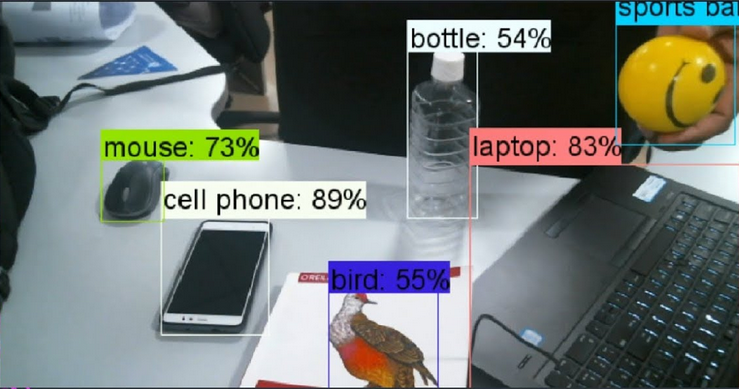
\includegraphics[width=0.5\textwidth]{project/images/ML-detec.png}
% 		\caption{Unity ML tutorial footage}
% 		\label{fig:mobile-neet}
% 	\end{figure}
%   As shown in Figure~\ref{fig:mobile-neet}. 
	With the help of material from different tutorials found over the web, it is possible to create a machine learning model for masking 
    However, it will be more efficient to use something more productive as Xception.
    In reality, this is the situation then speed matters more than accuracy.
    With QUT High-Performance Computer (HPC) Lyra, the training algorithm gets programmed for at least several days to build.
    As a result, only those, which produced maximum efficiency, were applied to report.
    The images above implements examples of~\cite{anuj_shah_tutorial_nodate} tutorial, with classifying several objects. For this case, only one will be enough.